\usetikzlibrary{calc}

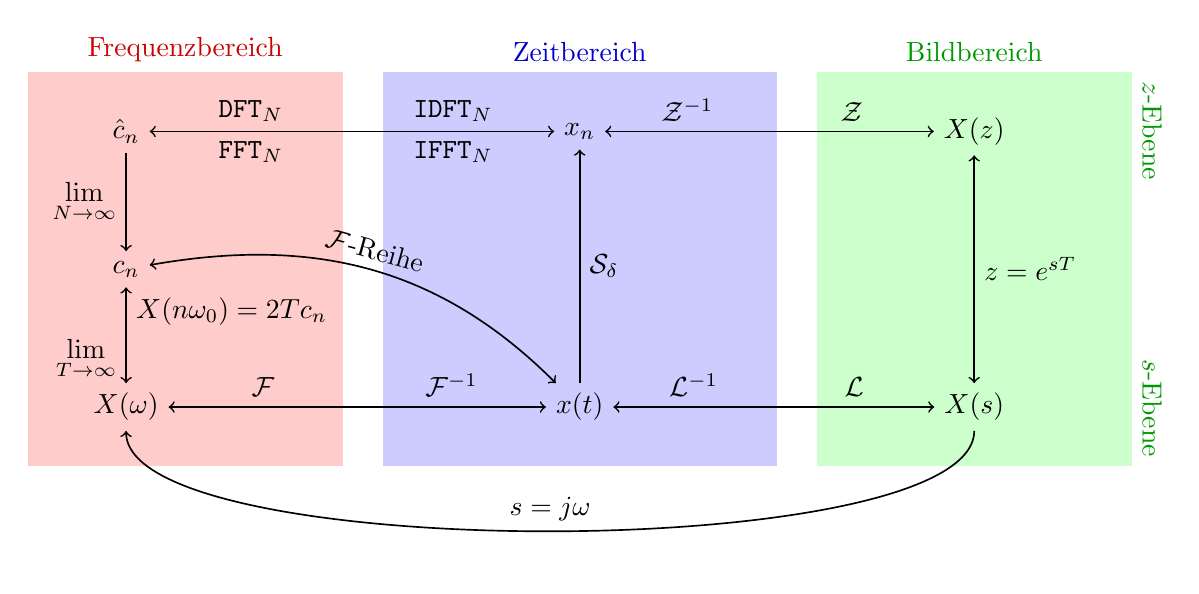
\begin{tikzpicture}[semithick]
  \node[fill=blue!20,
        minimum height=5cm,
        minimum width=5cm] (time) at (0,0) {};

  \node[fill=red!20,
        minimum height=5cm,
        minimum width=4cm,
        anchor=east] (freq) at (-3,0) {};

  \node[fill=green!20,
        %bottom color=green!30,
        %top color=teal!40,
        minimum height=5cm,
        minimum width=4cm,
        anchor=west] (cfreq) at (3,0) {};

  \node[blue!80!black, above] at (time.north) {Zeitbereich};
  \node[red!80!black, above] at (freq.north) {Frequenzbereich};
  \node[green!60!black, above] at (cfreq.north) {Bildbereich};

  \node[anchor=south west, rotate=-90, green!60!black]
    at (cfreq.north east) {\(z\)-Ebene};
  \node[anchor=south east, rotate=-90, green!60!black]
    at (cfreq.south east) {\(s\)-Ebene};

  \node (xt) at ($(time)  - (0,1.75)$) {\(x(t)\)};
  \node (xn) at ($(time)  + (0,1.75)$) {\(x_n\)};

  \node (Xo) at ($(freq)  + (-.75,-1.75)$) {\(X(\omega)\)};
  \node (Xn) at ($(freq)  + (-.75,1.75)$) {\(\hat{c}_n\)};
  \node (cn) at ($(freq)  + (-.75,0)$)    {\(c_n\)};

  \node (Xs) at ($(cfreq) - (0,1.75)$) {\(X(s)\)};
  \node (Xz) at ($(cfreq) + (0,1.75)$) {\(X(z)\)};

  \draw[->] (xt) to node[midway, right] {\(\mathcal{S}_\delta\)} (xn);

  \draw[<->] (Xs) to node[midway, right] {\(z=e^{sT}\)} (Xz);

  \draw[<->] (cn) to
    node[near end, left, anchor=east] {\(\displaystyle\lim_{T \to \infty}\)}
    node[near start, right] {\(X(n\omega_0) = 2Tc_n\)} (Xo);

  \draw[->] (Xn) to
    node[midway, left, anchor=east] {\(\displaystyle\lim_{N \to \infty}\)} (cn);

  \draw[<->] (xt) to[out=135, in=10]
    node[midway, sloped, above] {\(\mathcal{F}\)-Reihe} (cn);

  \draw[<->] (xt) to
    node[near end, above] {\(\mathcal{F}\)}
    node[near start, above] {\(\mathcal{F}^{-1}\)} (Xo);

  \draw[<->] (xt) to
    node[near end, above] {\(\mathcal{L}\)}
    node[near start, above] {\(\mathcal{L}^{-1}\)} (Xs);

  \draw[<->] (xn) to
    node[near end, above] {\(\mathtt{DFT}_N\)}
    node[near end, below] {\(\mathtt{FFT}_N\)}
    node[near start, above] {\(\mathtt{IDFT}_N\)}
    node[near start, below] {\(\mathtt{IFFT}_N\)} (Xn);

  \draw[<->] (xn) to
    node[near end, above] {\(\mathcal{Z}\)}
    node[near start, above] {\(\mathcal{Z}^{-1}\)} (Xz);

  \draw[->] (Xs) .. controls ($(Xs)-(0,2)$) and ($(Xo)-(0,2)$) ..
    node[midway, above] {\(s = j\omega\)} (Xo);
\end{tikzpicture}
